\section{Implementation \& Verification}\label{sec:implementation_and_verfication}

In this section the suggested structure in section \ref{sec:Structure}, implemented with the numerical solutions in section \ref{se:preissmann_scheme}-\ref{sec:concentrate}, is tested and verified.

The first part to be elaborated upon is the initialization.

 \subsection*{Initialization}

For the setup procedure of the simulation in list form, the specifications part shown in figure \ref{fig:sys_setup} needs to be defined. The parameters in the list for both pipe and tank can be seen in table \ref {tab:init_list}. 

\begin{enumerate} \label{tab:init_list}
	\item Pipe
	\begin{itemize}
		\item Length [m]
		\item Sections (Number of sections the pipe should be split in to)
		\item $\text{I}_\text{b}$ (Slope) [\textperthousand]
		\item $\Delta$x = Length/Sections [m]
		\item Diameter [meter]
		\item Theta (parameter used in Preissmann scheme)
		\item $\text{Q}_{\text{f}}$ (maximum flow found by Manning formula, see equation \ref{eq:qf_for_flow}) [$\text{m}^\text{3}/\text{s}$]
		\item Side/lateral inflow present 
		\item Section location in data 
	\end{itemize}
	\item Tank
	\begin{itemize}
		\item Size [$\text{m}^\text{3}$]
		\item Height [m]
		\item Area = Size / Height [$\text{m}^\text{2}$]
		\item Maximum outflow [$\text{m}^\text{3}/\text{s}$]
		\item Section location in data 
	\end{itemize}
	%b\caption{Table of needed parameters for pipe and tank}
\end{enumerate}

Some parameters can be found from others and is set to be calculated automatically. Furthermore an item is added that indicate in which section of the obtained data the specific output of the component is located. This item is given the number of the order in which the component appears in the list. To give an overview of the system to be simulated and to easily be able to locate specific parameters needed to simulate three structures is returned to the workspace. These are named ``pipe\_spec'', ``tank\_spec'' and ``sys\_setup''. The first two structures show the information shown in table \ref{tab:init_list} respectively and ``sys\_setup'' holds information of the  various parts indexed in the order it should be simulated. In figure \ref{fig:sys_setup_matlab}

\begin{figure}[H]
\centering
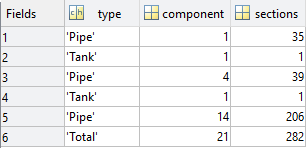
\includegraphics[width=0.5 \textwidth]{report/simulation/pictures/sys_setup_matlab.png}
\caption{Display of structure holding system setup information in MATLAB.}
\label{fig:sys_setup_matlab}
\end{figure}
